\documentclass[11pt,letterpaper]{article}
\input{../../preamble}
\usepackage{fullpage}
\usepackage{multicol}

\begin{document}
\flushleft
\begin{multicols}{2}

\begin{large}\textbf{Math 2554 Exam 1: Limits \\
date}\end{large}

\hfill\textbf{Name:  }\underline{\hspace{40ex}} %KEY\hspace{17ex}}

\vspace{.5in}

\end{multicols}

\pagestyle{empty}

\flushleft

You have 50 minutes to complete this exam.  Eyes on your own paper and good luck!

\begin{enumerate}
\item  \textbf{Definitions/Concepts.} 
\begin{enumerate}
\item (2.1) Suppose $s(t)$ is the position of an object moving along a line at a time $t\geq 0$.  What is the average velocity between the times $t=a$ and $t=b$?  What is the instantaneous velocity at $t=a$?  Which one is the slope of the secant line between the points $(a,s(a))$ and $(b,s(b))$ on the graph of $s$?  Which one gives the slope of the line tangent to the graph of $s$ at $(a,s(a))$? 

\item When $\lim_{x\to a}f(x)$ exists, it always equals $f(a)$.  (True or False?)

\item (2.5) The end behavior for $e^x$ and $e^{-x}$ (on the entire real line) and $\ln{x}$ (on the interval $(0,\infty)$) is given by
\begin{enumerate}
\item $\lim_{x\to\infty}e^x=$
\item $\lim_{x\to -\infty}e^x=$
\item $\lim_{x\to\infty}e^{-x}=$
\item $\lim_{x\to -\infty}e^{-x}=$
\item $\lim_{x\to\infty}\ln{x}=$
\item $\lim_{x\to 0+}\ln{x}=$
\end{enumerate}
\end{enumerate}

\item (2.4) The function $f(x)$ has a vertical asymptote at the line $x=a$ means at least one of the following conditions holds:
\begin{enumerate}
\item

\vspace{1pc}
\item 

\vspace{1pc}
\item 
\end{enumerate}

\item (2.6) Suppose a function $f(x)$ is continuous at the point $a$.  Why is it OK to plug in the value $x=a$ when computing $\lim_{x\to a}f(x)$ (Hint: What are the three conditions on the Continuity Checklist?)?

\end{enumerate}

\vspace{1pc}
\item \textbf{Questions/Problems.} 

\begin{enumerate}
\item (2.1/2.2) Sketch the graph of a function with the given properties.  You do not need to find a formula for the function.
\[f(1)=0,f(2)=4,f(3)=6,\lim_{x\to 2^-}f(x)=-3,\lim_{x\to 2^+}f(x)=5\]

\item The value of $\lim_{x\to 3}\frac{x^2-9}{x-3}$ does not exist. (t/f)

\item The value of $\lim_{x\to a}f(x)$ does not exist if $f(a)$ is undefined. (t/f)

\item (2.1/2.2) Use the graph of $g$ in the figure to find the following values, if they exist.  If a limit does not exist, explain why.

\vspace{-1pc}  
\begin{figure}[h]
\begin{center}
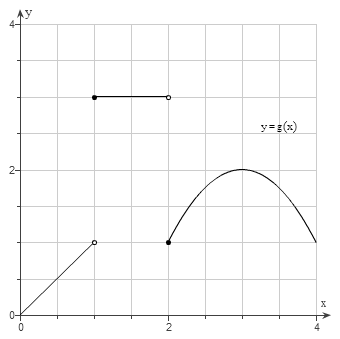
\includegraphics[scale=0.6]{Exam1pic.png}
\caption{$g$ (Briggs, W. and Cochran, L. \emph{Calculus: Early ranscendentals})}
\end{center}
\end{figure}

\begin{enumerate}
\item $g(1)$
\item $\lim_{x\to 1}g(x)$
\item $\lim_{x\to 2^+}g(x)$
\item $\lim_{x\to 1^-}g(x)$
\item $g(2)$
\item $g(3)$
\item $\lim_{x\to 1^+}g(x)$
\item $\lim_{x\to 2^-}g(x)$
\item $\lim_{x\to 3}g(x)$
\end{enumerate}

\item Using the figure as a guide, explain how the Squeeze Theorem can by used to compute $\lim_{x\to 0}x^2\sin(\frac{1}{x})$, and then say what the limit is.
\vspace{-1pc}  
\begin{figure}[h]
\begin{center}
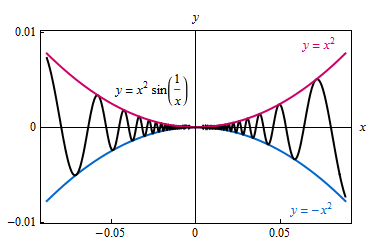
\includegraphics[scale=0.8]{Exam1pic2.png}
\caption{(Briggs, W. and Cochran, L. \emph{Calculus: Early Transcendentals})}
\end{center}
\end{figure}

\item (CHALLENGE) Suppose a spaceship is traveling at velocity $v$, relative to an observer.  Say the length of the spaceship is $L_0$.  To the observer, the ship appears to have a smaller length, given by the Lorentz contraction formula:
\[\text{length to the observer}=L_0\sqrt{1-\frac{v^2}{c^2}},\]
where $c$ is the speed of light.
\begin{enumerate}
\item If $v=0.5c$, i.e., the ship is traveling at half the speed of light, then what is the length of the ship to the observer?
\item If the ship is traveling 75\% of the speed of light then how long does the ship look to the observer?
\item Compute $\lim_{v\to c^-}L_0\sqrt{1-\frac{v^2}{c^2}}$.  What is physically interesting about this limit?
\end{enumerate}

\item (2.3) Suppose $\lim_{x\to 1}f(x)=4$.  What is $\lim_{x\to -1}f(x^2)$?  (Hint: There is another limit law that says how to compute this limit.)

\item (2.3/2.4) Suppose $g(x)=\begin{cases}\frac{x-5}{x} & x\neq 0 \\
	0 & x=0 \end{cases}$.  Evaluate 
	\begin{enumerate}
	\item $\lim_{x\to 0^+}g(x)$.  Make sure your justification involves determining the sign of the numerator and denominator for $x$-values slightly larger than 0.
	\item $\lim_{x\to 0^-}g(x)$.  Make sure your justification involves determining the sign of the numerator and denominator for $x$-values slightly smaller than 0.
	\item $\lim_{x\to 0}g(x)$.
	\item $g(0)$.
	\end{enumerate}
\item (2.3/2.4) Suppose $h(x)=\begin{cases}\frac{x-5}{x} & x\lneq 0 \\
	0 & x\geq 0 \end{cases}$.  Evaluate 
	\begin{enumerate}
	\item $\lim_{x\to 0^+}h(x)$.  
	\item $\lim_{x\to 0^-}h(x)$.  Make sure your justification involves determining the sign of the numerator and denominator for $x$-values slightly smaller than 0.
	\item $\lim_{x\to 0}h(x)$.
	\item $h(0)$.
	\item Does $h$ have a vertical asymptote at the line $x=0$?
	\end{enumerate}	
\item (2.4) The graph of $f$ in the figure has vertical asymptotes at $x=1$ and $x=2$.  Find the following limits, if possible.  If not possible, then say so and why.
\vspace{-1pc}  
\begin{figure}[h]
\begin{center}
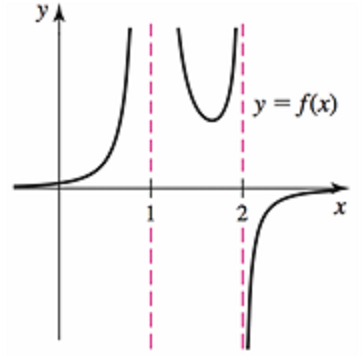
\includegraphics[scale=0.6]{Exam1pic3.png}
\caption{(Briggs, W. and Cochran, L. \emph{Calculus: Early Transcendentals})}
\end{center}
\end{figure}
\begin{enumerate}
\item $\lim_{x\to 1^-}f(x)$
\item $\lim_{x\to 1^+}f(x)$
\item $\lim_{x\to 1}f(x)$
\item $\lim_{x\to 2^-}f(x)$
\item $\lim_{x\to 2^+}f(x)$
\item $\lim_{x\to 2}f(x)$
\end{enumerate}
	
\item (2.4) Sketch a possible graph of a function $f$, together with vertical asymptotes, satisfying all of the following conditions.
\begin{enumerate}
\item $f(1)=0$
\item $f(3)$ is undefined
\item $\lim_{x\to 3}f(x)=1$
\item $\lim_{x\to 0^+}=-\infty$
\item $\lim_{x\to 2}f(x)=\infty$
\item $\lim_{x\to 4^-}f(x)=\infty$
\end{enumerate}	

\item (2.1/3.1) Given the graph of $f$ in the following figures, find the slope of the secant line that passes through $(0,0)$ and $(h,f(h))$, in terms of $h$, for $h>0$ and $h<0$.  Then calculate the limit of that slope as $h\to 0^+$ and as $h\to 0^-$.  What does this tell you about the tangent line to the curve at $(0,0)$?  Why doesn't $f$ itself have a vertical asymptote in either of these cases?
\begin{enumerate}
\item $f(x)=x^{\frac{1}{3}}$
\vspace{-1pc}  
\begin{figure}[h]
\begin{center}
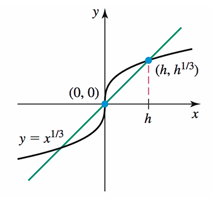
\includegraphics[scale=0.8]{Exam1pic4.png}
\caption{(Briggs, W. and Cochran, L. \emph{Calculus: Early Transcendentals})}
\end{center}
\end{figure}

\item $f(x)=x^{\frac{2}{3}}$
\vspace{-1pc}  
\begin{figure}[h]
\begin{center}
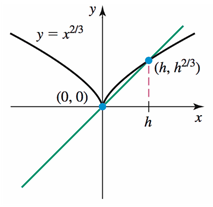
\includegraphics[scale=0.8]{Exam1pic5.png}
\caption{(Briggs, W. and Cochran, L. \emph{Calculus: Early Transcendentals})}
\end{center}
\end{figure}
\end{enumerate}

\item (up to 2.5) Sketch a possible graph of a function $f$ that satisfies all of the given conditions.  Be sure to identify all the vertical and horizontal asymptotes.
\begin{enumerate}
\item $f(-1)=-2$
\item $f(1)=2$
\item $f(0)=0$
\item $\lim_{x\to\infty}f(x)=1$
\item $\lim_{x\to -\infty}f(x)=-1$
\end{enumerate}

\item (2.4/2.5) For each function $f(x)$, evaluate $\lim_{x\to\infty}f(x)$ and $\lim_{x\to -\infty}f(x)$, and then identify any horizontal asymptotes.  Next, find the vertical asymptotes.  For each vertical asymptote $x=a$, evaluate $\lim_{x\to a^-}f(x)$ and $\lim_{x\to a^+}f(x)$.
\begin{enumerate}
\item $f(x)=\frac{x^2-4x+3}{x-1}$
\item $f(x)=\frac{\sqrt{16x^4+64x^2}+x^2}{2x^2-4}$
\item $f(x)=\frac{x^2-4}{x(x-2)}$
\end{enumerate}

\item (2.6) Does the function 
\[f(x)=2x^5-8x^3+5x^2+3x-5\] 
cross the horizontal line $y=-4$ for some $x$ in the interval $\left[0,1\right]$?  (Yes, it does.)  Justify your answer, and in particular, mention any important theorems you use and why they apply in this situation. 
\end{enumerate}

\item (2.3) (ChAlLeNgE pRoBlEm) Suppose $\lim_{x\to 1}f(x)=4$.  What is $\lim_{x\to -1}f(x^2)$? 

\vspace{1pc}
\item \textbf{Computations/Algebra.} 

\begin{enumerate}
\item (2.3) $\lim_{x\to 4}(3x-7)$
\item (2.3) $\lim_{x\to -5}\pi$
\item (2.3) $\lim_{x\to -5}2$
\item (2.3) Suppose $\lim_{x\to 1}f(x)=8,\lim_{x\to 1}g(x)=3$, and $\lim_{x\to 1}h(x)=2$.  Compute the following limits and state the limit laws used (and why you are allowed to use them in that instance, if there is a caveat) to justify your computations.  If the limit does not exist then say so.
\begin{enumerate}
\item $\lim_{x\to 1}4f(x)$
\item $\lim_{x\to 1}\frac{f(x)g(x)}{h(x)}$
\item $\lim_{x\to 1}\sqrt[3]{f(x)g(x)+3}$
\item $\lim_{x\to 1}(2x^3-3x^2+4x+5)$
\item $\lim_{x\to 1}\left(x^2-x\right)^5$
\item $\lim_{x\to 3^-}\sqrt{\frac{x-3}{2-x}}$
\item $\lim_{x\to 3}\sqrt{\frac{x-3}{2-x}}$
\item $\lim_{x\to 3^+}\sqrt{\frac{x-3}{2-x}}$
\item $\lim_{x\to -b}\frac{(x+b)^7+(x+b)^{10}}{4(x+b)}$
\item $\lim_{t\to a}\frac{\sqrt{3t+1}-\sqrt{3a-1}}{t-a}$
\item $\lim_{x\to 0}\frac{a-\sqrt{a^2-x^2}}{x^2}$
\item $\lim_{x\to 2}\left(\frac{1}{x-2}-\frac{2}{x^2-2x}\right)$
\item $\lim_{x\to c}\frac{x^2-2cx+c^2}{x-c}$
\item $\lim_{x\to\infty}\frac{2x}{x+1}$
\item $\lim_{x\to -\infty}\left(5+\frac{100}{x}+\frac{\sin^4x^3}{x^2}\right)$
\item $\lim_{x\to -\infty}\left(3x^7+x^2\right)$
\item $\lim_{x\to\infty}-12x^{-5}$
\end{enumerate}


\end{enumerate}


\end{document}


